% Four demo diagrams, one per page. Build: tectonic diagrams.tex, then scripts in README export PNGs.
\documentclass[tikz,border=14pt]{standalone}
\usepackage[T1]{fontenc}
\usepackage[scaled]{helvet}
\renewcommand{\familydefault}{\sfdefault}
\usepackage{xcolor}
\usetikzlibrary{arrows.meta,positioning,fit,backgrounds,calc,shapes.geometric}
\definecolor{ink}{HTML}{1F2A44}
\definecolor{acc}{HTML}{0F7B6C}
\definecolor{warn}{HTML}{B5462E}
\definecolor{gold}{HTML}{D9A441}
\definecolor{soft}{HTML}{E8F3F1}
\definecolor{softw}{HTML}{F7E9E5}
\definecolor{softg}{HTML}{FBF3E0}
\definecolor{grey}{HTML}{5B6475}
\tikzset{
  b/.style={draw=ink,rounded corners=4pt,fill=soft,align=center,font=\small,inner sep=5pt,minimum height=11mm},
  bw/.style={b,fill=softw,draw=warn},
  bg/.style={b,fill=softg,draw=gold},
  bi/.style={b,fill=ink,text=white,draw=ink},
  ba/.style={b,fill=acc,text=white,draw=acc},
  bp/.style={b,fill=white,draw=black!30},
  a/.style={-{Stealth[length=2.6mm]},thick,draw=ink},
  aw/.style={a,draw=warn},
  l/.style={font=\footnotesize,text=grey},
  title/.style={font=\bfseries\LARGE,text=ink,anchor=west},
  sub/.style={font=\normalsize,text=grey,anchor=west},
  tt/.style={font=\ttfamily\footnotesize},
}
\begin{document}

%% ---------------------------------------------------------------- 1. Where are we
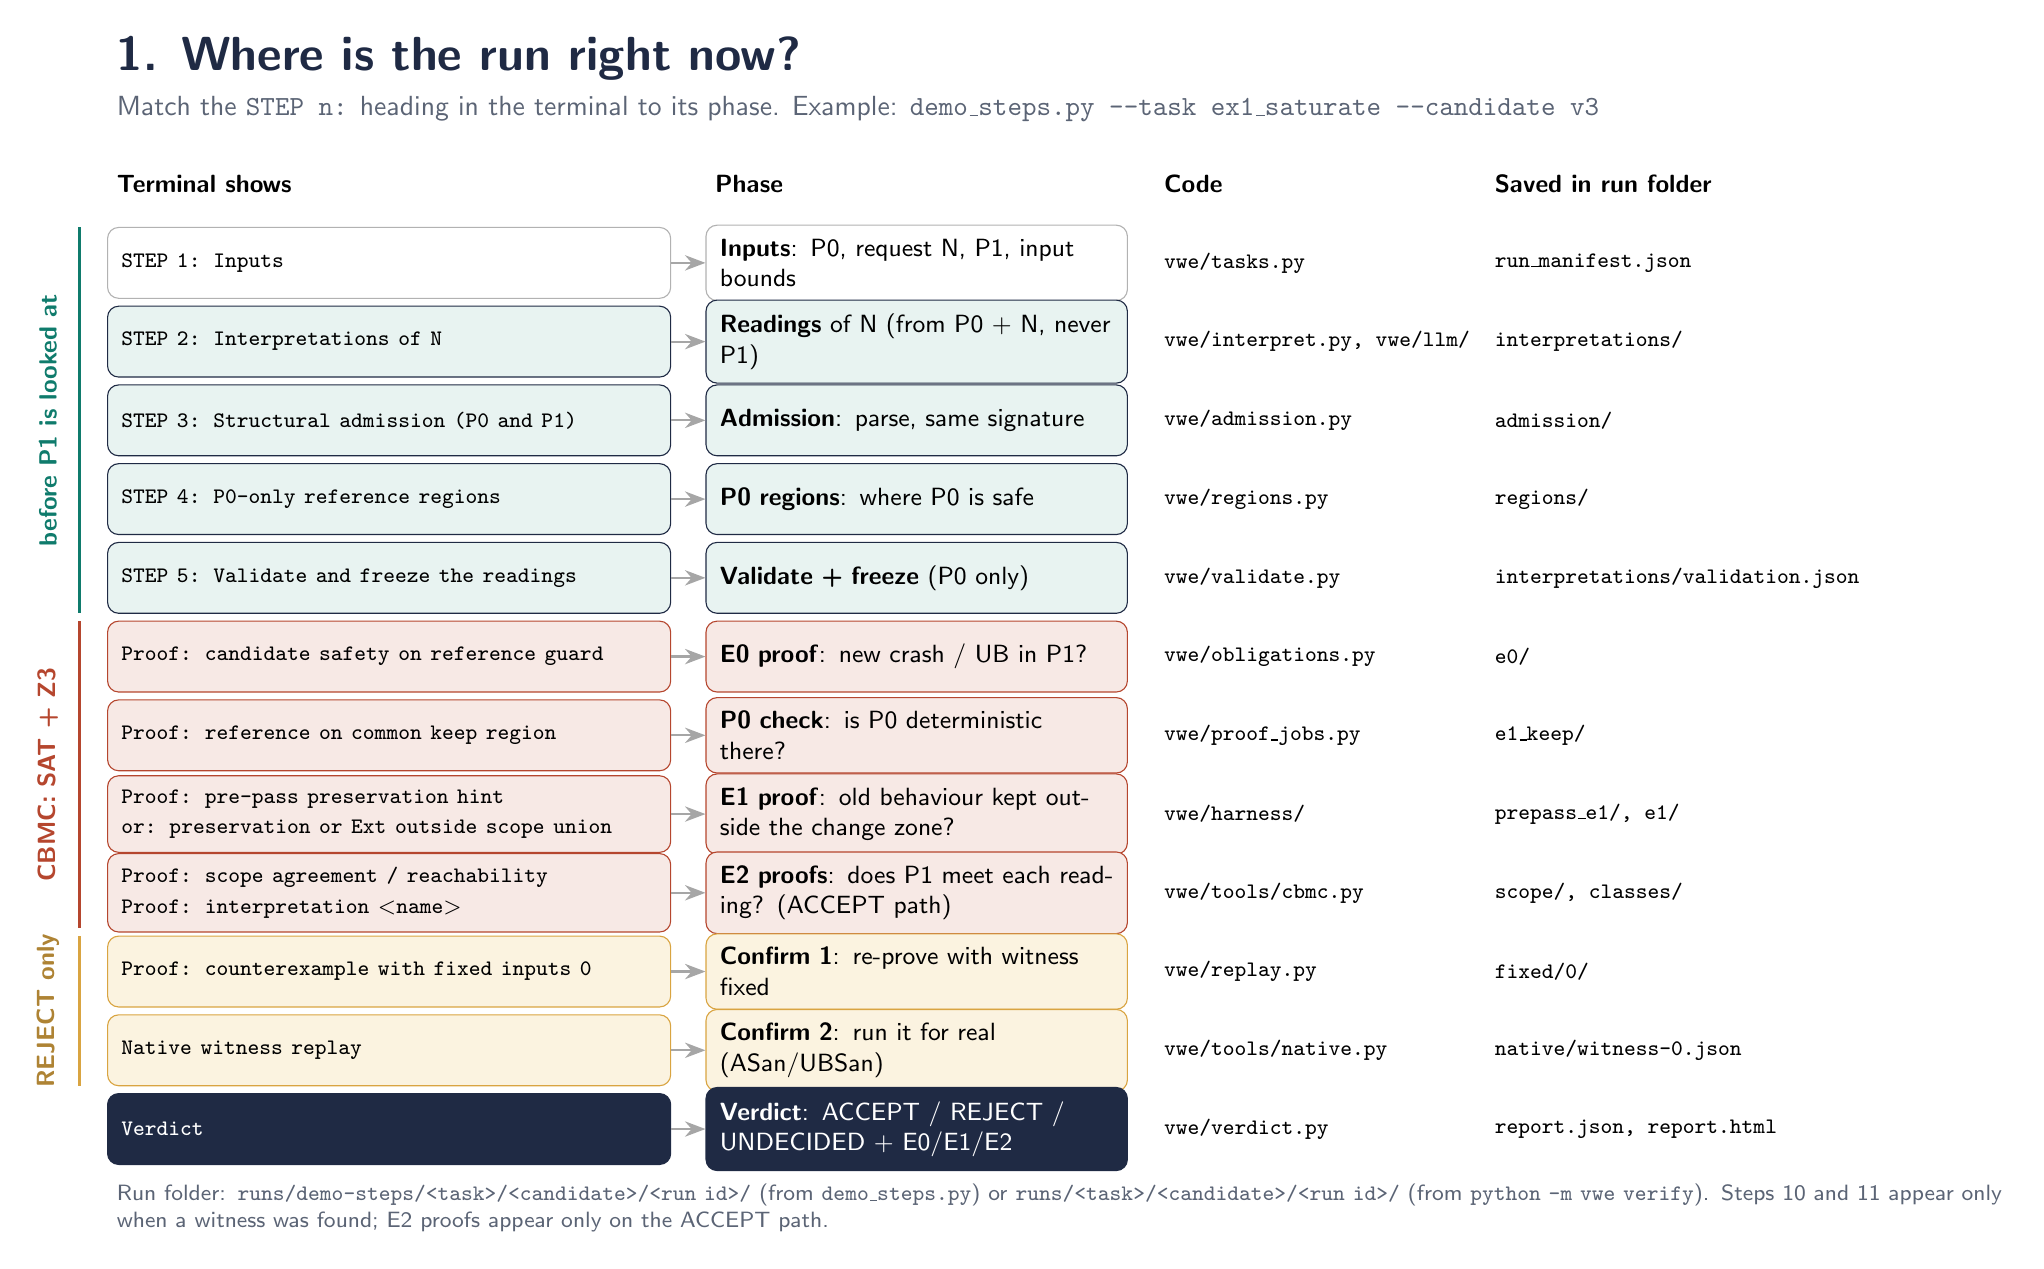
\begin{tikzpicture}[x=1cm,y=1cm]
\node[title] at (0,1.6) {1. Where is the run right now?};
\node[sub] at (0,0.95) {Match the \texttt{STEP n:} heading in the terminal to its phase. Example: \texttt{demo\_steps.py --task ex1\_saturate --candidate v3}};
% columns
\node[font=\bfseries\small,anchor=west] at (0,0) {Terminal shows};
\node[font=\bfseries\small,anchor=west] at (7.6,0) {Phase};
\node[font=\bfseries\small,anchor=west] at (13.3,0) {Code};
\node[font=\bfseries\small,anchor=west] at (17.5,0) {Saved in run folder};
\def\row#1#2#3#4#5#6{%
  \node[#6,minimum width=7cm,text width=6.8cm,align=left,anchor=west,minimum height=9mm] (t#1) at (0,#2) {\ttfamily\footnotesize #3};
  \node[#6,minimum width=5.2cm,text width=5cm,align=left,anchor=west,minimum height=9mm] (p#1) at (7.6,#2) {#4};
  \node[anchor=west,font=\ttfamily\footnotesize] at (13.3,#2) {#5};
}
\row{1}{-1.0}{STEP 1: Inputs}{\textbf{Inputs}: P0, request N, P1, input bounds}{vwe/tasks.py}{bp}
\node[anchor=west,font=\ttfamily\footnotesize] at (17.5,-1.0) {run\_manifest.json};
\row{2}{-2.0}{STEP 2: Interpretations of N}{\textbf{Readings} of N (from P0 + N, never P1)}{vwe/interpret.py, vwe/llm/}{b}
\node[anchor=west,font=\ttfamily\footnotesize] at (17.5,-2.0) {interpretations/};
\row{3}{-3.0}{STEP 3: Structural admission (P0 and P1)}{\textbf{Admission}: parse, same signature}{vwe/admission.py}{b}
\node[anchor=west,font=\ttfamily\footnotesize] at (17.5,-3.0) {admission/};
\row{4}{-4.0}{STEP 4: P0-only reference regions}{\textbf{P0 regions}: where P0 is safe}{vwe/regions.py}{b}
\node[anchor=west,font=\ttfamily\footnotesize] at (17.5,-4.0) {regions/};
\row{5}{-5.0}{STEP 5: Validate and freeze the readings}{\textbf{Validate + freeze} (P0 only)}{vwe/validate.py}{b}
\node[anchor=west,font=\ttfamily\footnotesize] at (17.5,-5.0) {interpretations/validation.json};
\row{6}{-6.0}{Proof: candidate safety on reference guard}{\textbf{E0 proof}: new crash / UB in P1?}{vwe/obligations.py}{bw}
\node[anchor=west,font=\ttfamily\footnotesize] at (17.5,-6.0) {e0/};
\row{7}{-7.0}{Proof: reference on common keep region}{\textbf{P0 check}: is P0 deterministic there?}{vwe/proof\_jobs.py}{bw}
\node[anchor=west,font=\ttfamily\footnotesize] at (17.5,-7.0) {e1\_keep/};
\row{8}{-8.0}{Proof: pre-pass preservation hint\\or: preservation or Ext outside scope union}{\textbf{E1 proof}: old behaviour kept outside the change zone?}{vwe/harness/}{bw}
\node[anchor=west,font=\ttfamily\footnotesize] at (17.5,-8.0) {prepass\_e1/, e1/};
\row{9}{-9.0}{Proof: scope agreement / reachability\\Proof: interpretation \textless name\textgreater}{\textbf{E2 proofs}: does P1 meet each reading? (ACCEPT path)}{vwe/tools/cbmc.py}{bw}
\node[anchor=west,font=\ttfamily\footnotesize] at (17.5,-9.0) {scope/, classes/};
\row{10}{-10.0}{Proof: counterexample with fixed inputs 0}{\textbf{Confirm 1}: re-prove with witness fixed}{vwe/replay.py}{bg}
\node[anchor=west,font=\ttfamily\footnotesize] at (17.5,-10.0) {fixed/0/};
\row{11}{-11.0}{Native witness replay}{\textbf{Confirm 2}: run it for real (ASan/UBSan)}{vwe/tools/native.py}{bg}
\node[anchor=west,font=\ttfamily\footnotesize] at (17.5,-11.0) {native/witness-0.json};
\row{12}{-12.0}{Verdict}{\textbf{Verdict}: ACCEPT / REJECT / UNDECIDED + E0/E1/E2}{vwe/verdict.py}{bi}
\node[anchor=west,font=\ttfamily\footnotesize] at (17.5,-12.0) {report.json, report.html};
\foreach \i in {1,...,12} {\draw[a,draw=black!35] (t\i.east) -- (p\i.west);}
% brackets
\draw[thick,draw=acc] (-0.35,-0.55) -- (-0.35,-5.45);
\node[rotate=90,font=\bfseries\small,text=acc] at (-0.75,-3.0) {before P1 is looked at};
\draw[thick,draw=warn] (-0.35,-5.55) -- (-0.35,-9.45);
\node[rotate=90,font=\bfseries\small,text=warn] at (-0.75,-7.5) {CBMC: SAT + Z3};
\draw[thick,draw=gold] (-0.35,-9.55) -- (-0.35,-11.45);
\node[rotate=90,font=\bfseries\small,text=gold!80!black] at (-0.75,-10.5) {REJECT only};
\node[l,anchor=west,text width=24cm] at (0,-13.0) {Run folder: \texttt{runs/demo-steps/<task>/<candidate>/<run id>/} (from \texttt{demo\_steps.py}) or \texttt{runs/<task>/<candidate>/<run id>/} (from \texttt{python -m vwe verify}). Steps 10 and 11 appear only when a witness was found; E2 proofs appear only on the ACCEPT path.};
\end{tikzpicture}

%% ---------------------------------------------------------------- 2. Inside one proof
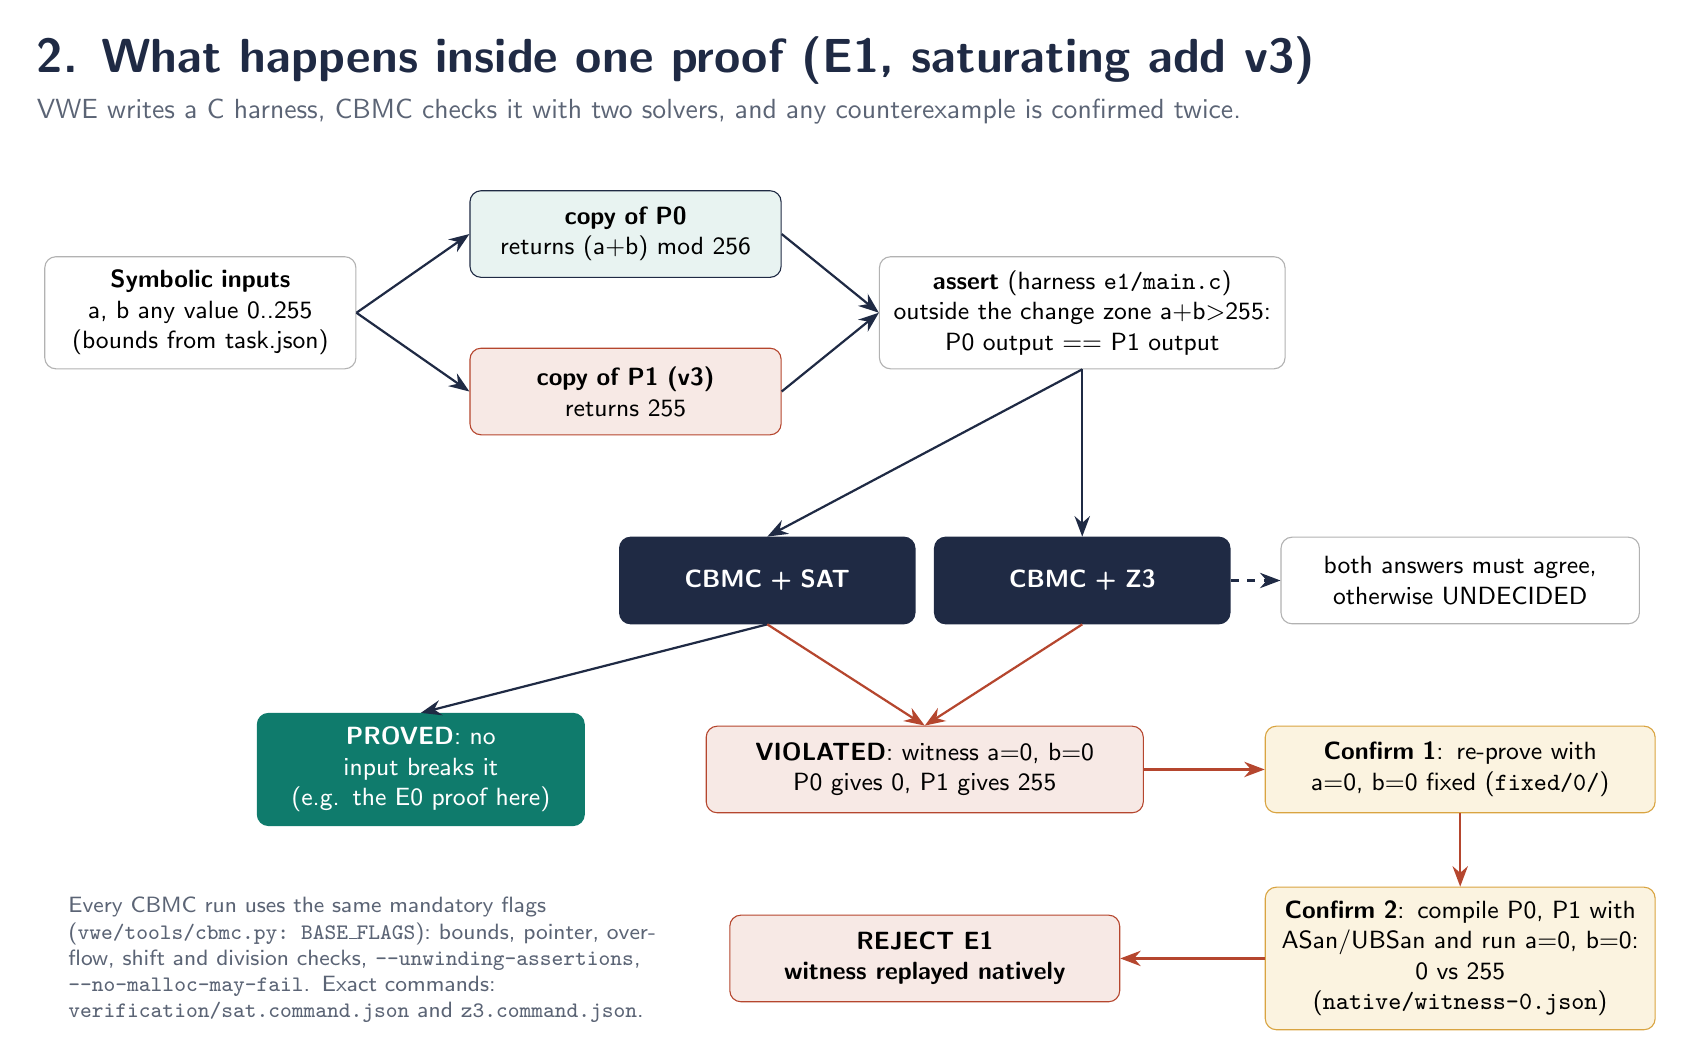
\begin{tikzpicture}[x=1cm,y=1cm]
\node[title] at (0,3.2) {2. What happens inside one proof (E1, saturating add v3)};
\node[sub] at (0,2.55) {VWE writes a C harness, CBMC checks it with two solvers, and any counterexample is confirmed twice.};
\node[bp,text width=3.6cm] (in) at (2.2,0) {\textbf{Symbolic inputs}\\a, b any value 0..255\\(bounds from task.json)};
\node[b,text width=3.6cm] (p0) at (7.6,1.0) {\textbf{copy of P0}\\returns (a+b) mod 256};
\node[bw,text width=3.6cm] (p1) at (7.6,-1.0) {\textbf{copy of P1 (v3)}\\returns 255};
\node[bp,text width=4.8cm] (as) at (13.4,0) {\textbf{assert} (harness \texttt{e1/main.c})\\outside the change zone a+b$>$255:\\P0 output == P1 output};
\draw[a] (in.east) -- (p0.west); \draw[a] (in.east) -- (p1.west); \draw[a] (p0.east) -- (as.west); \draw[a] (p1.east) -- (as.west);
\node[bi,text width=3.4cm] (sat) at (9.4,-3.4) {\textbf{CBMC + SAT}};
\node[bi,text width=3.4cm] (z3) at (13.4,-3.4) {\textbf{CBMC + Z3}};
\node[bp,text width=4.2cm] (agree) at (18.2,-3.4) {both answers must agree,\\otherwise UNDECIDED};
\draw[a] (as.south) -- (sat.north); \draw[a] (as.south) -- (z3.north); \draw[a,dashed] (z3.east) -- (agree.west);
\node[ba,text width=3.8cm] (ok) at (5.0,-5.8) {\textbf{PROVED}: no input breaks it\\(e.g. the E0 proof here)};
\node[bw,text width=5.2cm] (bad) at (11.4,-5.8) {\textbf{VIOLATED}: witness a=0, b=0\\P0 gives 0, P1 gives 255};
\draw[a] (sat.south) -- (ok.north); \draw[aw] (sat.south) -- (bad.north); \draw[aw] (z3.south) -- (bad.north);
\node[bg,text width=4.6cm] (fx) at (18.2,-5.8) {\textbf{Confirm 1}: re-prove with\\a=0, b=0 fixed (\texttt{fixed/0/})};
\node[bg,text width=4.6cm] (nat) at (18.2,-8.2) {\textbf{Confirm 2}: compile P0, P1 with\\ASan/UBSan and run a=0, b=0:\\0 vs 255 (\texttt{native/witness-0.json})};
\node[bw,text width=4.6cm,font=\small\bfseries] (rej) at (11.4,-8.2) {REJECT E1\\witness replayed natively};
\draw[aw] (bad.east) -- (fx.west); \draw[aw] (fx.south) -- (nat.north); \draw[aw] (nat.west) -- (rej.east);
\node[l,anchor=north west,text width=8.6cm] at (0.4,-7.3) {Every CBMC run uses the same mandatory flags (\texttt{vwe/tools/cbmc.py: BASE\_FLAGS}): bounds, pointer, overflow, shift and division checks, \texttt{--unwinding-assertions}, \texttt{--no-malloc-may-fail}. Exact commands: \texttt{verification/sat.command.json} and \texttt{z3.command.json}.};
\end{tikzpicture}

%% ---------------------------------------------------------------- 3. Verdict rules
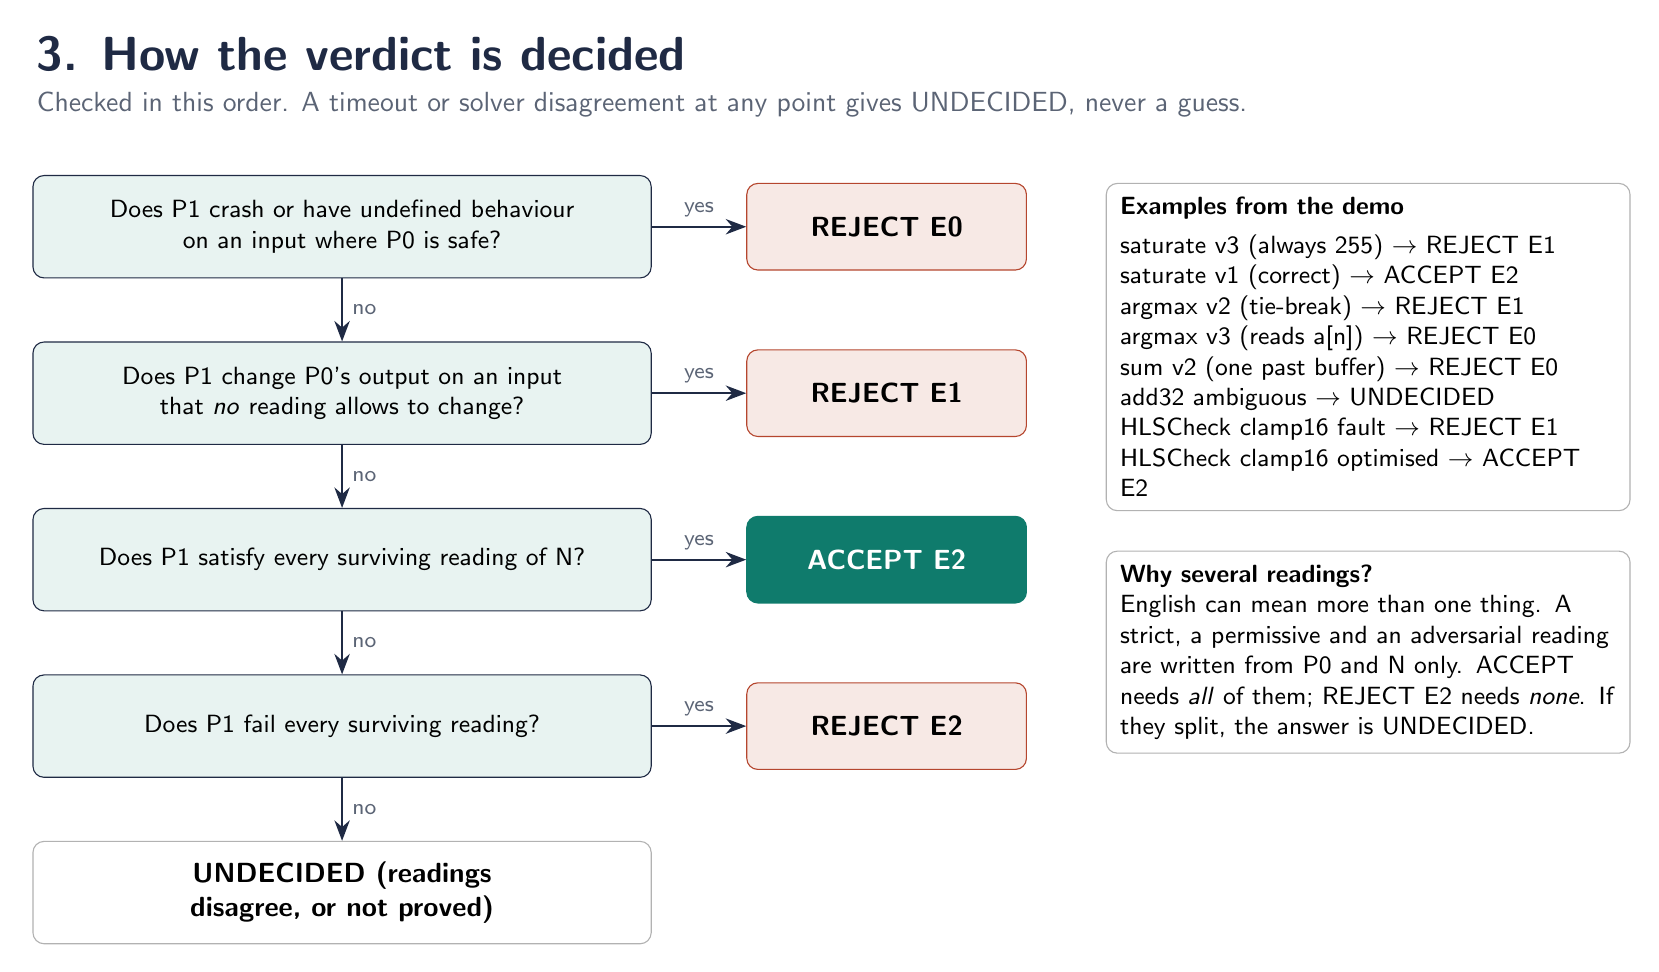
\begin{tikzpicture}[node distance=8mm and 12mm]
\node[title] at (-1.5,1.6) {3. How the verdict is decided};
\node[sub] at (-1.5,0.95) {Checked in this order. A timeout or solver disagreement at any point gives UNDECIDED, never a guess.};
\node[b,text width=7.5cm,minimum height=13mm] (q0) at (2.5,-0.6) {Does P1 crash or have undefined behaviour\\on an input where P0 is safe?};
\node[bw,text width=3.2cm,right=of q0,font=\bfseries] (r0) {REJECT E0};
\node[b,text width=7.5cm,minimum height=13mm,below=of q0] (q1) {Does P1 change P0's output on an input\\that \emph{no} reading allows to change?};
\node[bw,text width=3.2cm,right=of q1,font=\bfseries] (r1) {REJECT E1};
\node[b,text width=7.5cm,minimum height=13mm,below=of q1] (q2) {Does P1 satisfy every surviving reading of N?};
\node[ba,text width=3.2cm,right=of q2,font=\bfseries] (r2) {ACCEPT E2};
\node[b,text width=7.5cm,minimum height=13mm,below=of q2] (q3) {Does P1 fail every surviving reading?};
\node[bw,text width=3.2cm,right=of q3,font=\bfseries] (r3) {REJECT E2};
\node[bp,text width=7.5cm,minimum height=13mm,below=of q3,font=\bfseries] (u) {UNDECIDED (readings disagree, or not proved)};
\foreach \q/\r in {q0/r0,q1/r1,q2/r2,q3/r3} {\draw[a] (\q) -- node[l,above]{yes} (\r);}
\foreach \x/\y in {q0/q1,q1/q2,q2/q3,q3/u} {\draw[a] (\x) -- node[l,right]{no} (\y);}
\node[bp,text width=6.3cm,align=left,anchor=north west] (ex) at ($(r0.north east)+(1.0,0)$) {\textbf{Examples from the demo}\\[3pt]
saturate v3 (always 255) $\to$ REJECT E1\\
saturate v1 (correct) $\to$ ACCEPT E2\\
argmax v2 (tie-break) $\to$ REJECT E1\\
argmax v3 (reads a[n]) $\to$ REJECT E0\\
sum v2 (one past buffer) $\to$ REJECT E0\\
add32 ambiguous $\to$ UNDECIDED\\
HLSCheck clamp16 fault $\to$ REJECT E1\\
HLSCheck clamp16 optimised $\to$ ACCEPT E2};
\node[bp,text width=6.3cm,align=left,anchor=north west] at ($(ex.south west)+(0,-0.5)$) {\textbf{Why several readings?}\\English can mean more than one thing. A
strict, a permissive and an adversarial reading are written from P0 and N only. ACCEPT needs \emph{all} of them; REJECT E2 needs
\emph{none}. If they split, the answer is UNDECIDED.};
\end{tikzpicture}

%% ---------------------------------------------------------------- 4. Repo map
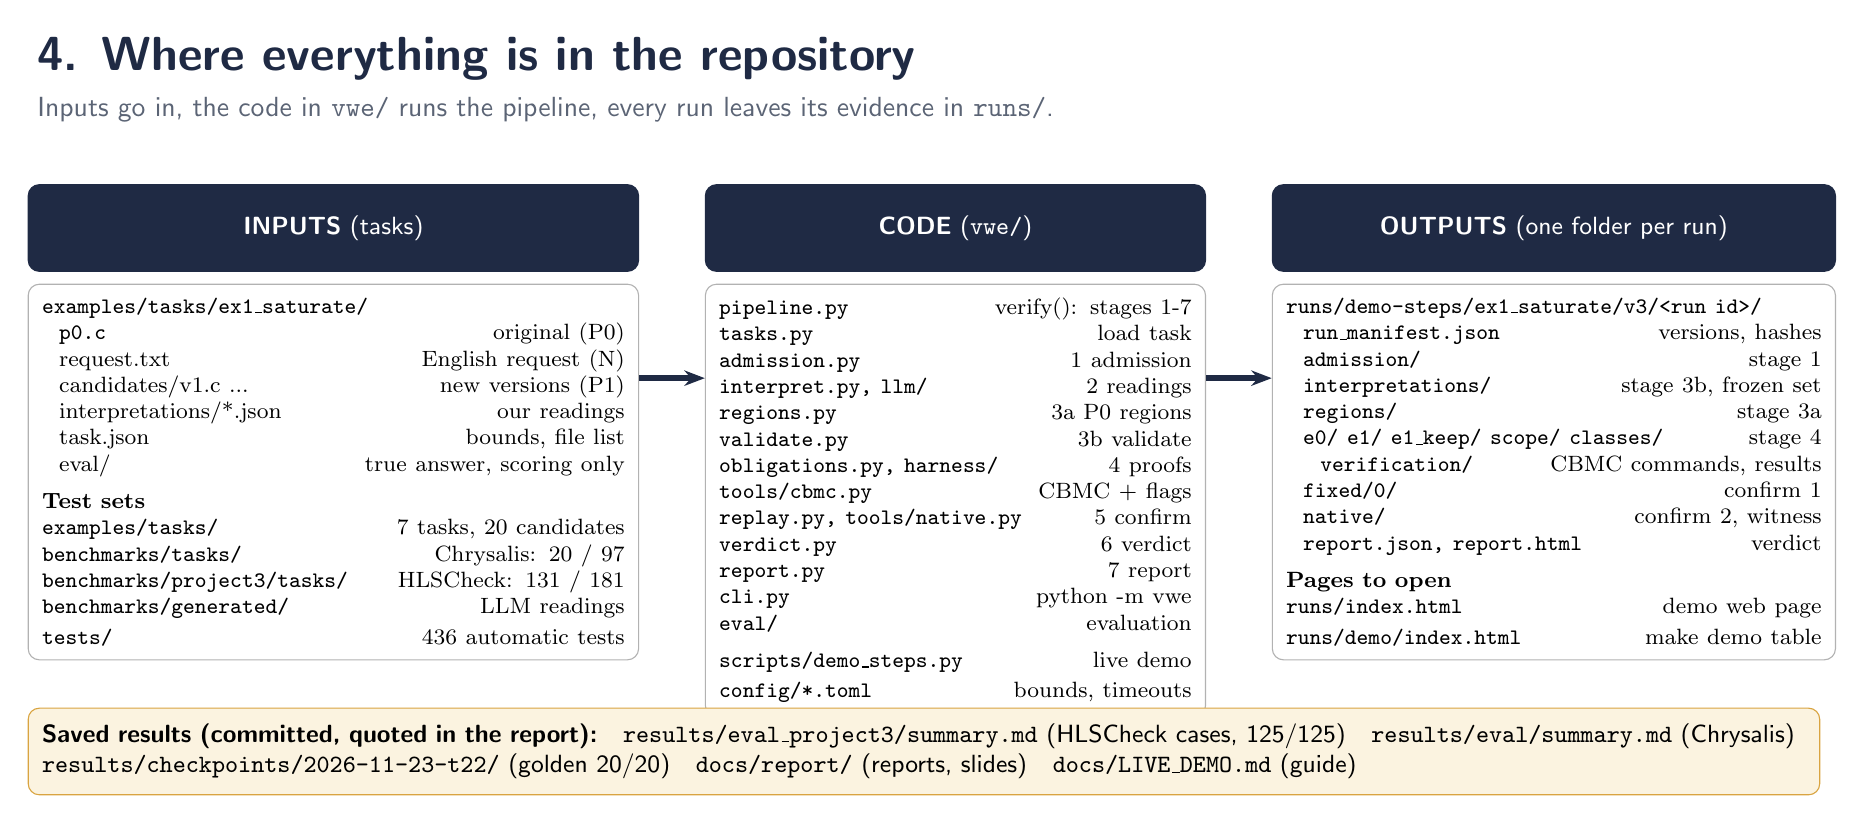
\begin{tikzpicture}[node distance=6mm and 8mm]
\node[title] at (0,1.6) {4. Where everything is in the repository};
\node[sub] at (0,0.95) {Inputs go in, the code in \texttt{vwe/} runs the pipeline, every run leaves its evidence in \texttt{runs/}.};
% inputs
\node[bi,text width=7.4cm,anchor=north west] (ih) at (0,0) {\textbf{INPUTS} (tasks)};
\node[bp,text width=7.4cm,align=left,anchor=north west] (ib) at ($(ih.south west)+(0,-0.15)$) {\tt\footnotesize
examples/tasks/ex1\_saturate/\\
\ \ p0.c\hfill\rm original (P0)\\
\ \ request.txt\hfill\rm English request (N)\\
\ \ candidates/v1.c ...\hfill\rm new versions (P1)\\
\ \ interpretations/*.json\hfill\rm our readings\\
\ \ task.json\hfill\rm bounds, file list\\
\ \ eval/\hfill\rm true answer, scoring only\\[4pt]
\rm\bfseries Test sets\\ \tt
examples/tasks/\hfill\rm 7 tasks, 20 candidates\\ \tt
benchmarks/tasks/\hfill\rm Chrysalis: 20 / 97\\ \tt
benchmarks/project3/tasks/\hfill\rm HLSCheck: 131 / 181\\ \tt
benchmarks/generated/\hfill\rm LLM readings\\ \tt
tests/\hfill\rm 436 automatic tests};
% code
\node[bi,text width=6.0cm,anchor=north west] (ch) at (8.6,0) {\textbf{CODE} (\texttt{vwe/})};
\node[bp,text width=6.0cm,align=left,anchor=north west] (cb) at ($(ch.south west)+(0,-0.15)$) {\tt\footnotesize
pipeline.py\hfill\rm verify(): stages 1-7\\ \tt
tasks.py\hfill\rm load task\\ \tt
admission.py\hfill\rm 1 admission\\ \tt
interpret.py, llm/\hfill\rm 2 readings\\ \tt
regions.py\hfill\rm 3a P0 regions\\ \tt
validate.py\hfill\rm 3b validate\\ \tt
obligations.py, harness/\hfill\rm 4 proofs\\ \tt
tools/cbmc.py\hfill\rm CBMC + flags\\ \tt
replay.py, tools/native.py\hfill\rm 5 confirm\\ \tt
verdict.py\hfill\rm 6 verdict\\ \tt
report.py\hfill\rm 7 report\\ \tt
cli.py\hfill\rm python -m vwe\\ \tt
eval/\hfill\rm evaluation\\[4pt] \tt
scripts/demo\_steps.py\hfill\rm live demo\\ \tt
config/*.toml\hfill\rm bounds, timeouts};
% outputs
\node[bi,text width=6.8cm,anchor=north west] (oh) at (15.8,0) {\textbf{OUTPUTS} (one folder per run)};
\node[bp,text width=6.8cm,align=left,anchor=north west] (ob) at ($(oh.south west)+(0,-0.15)$) {\tt\footnotesize
runs/demo-steps/ex1\_saturate/v3/<run id>/\\
\ \ run\_manifest.json\hfill\rm versions, hashes\\ \tt
\ \ admission/\hfill\rm stage 1\\ \tt
\ \ interpretations/\hfill\rm stage 3b, frozen set\\ \tt
\ \ regions/\hfill\rm stage 3a\\ \tt
\ \ e0/ e1/ e1\_keep/ scope/ classes/\hfill\rm stage 4\\ \tt
\ \ \ \ verification/\hfill\rm CBMC commands, results\\ \tt
\ \ fixed/0/\hfill\rm confirm 1\\ \tt
\ \ native/\hfill\rm confirm 2, witness\\ \tt
\ \ report.json, report.html\hfill\rm verdict\\[4pt]
\rm\bfseries Pages to open\\ \tt
runs/index.html\hfill\rm demo web page\\ \tt
runs/demo/index.html\hfill\rm make demo table};
\draw[a,line width=2pt] ($(ib.north east)+(0,-1.2)$) -- ($(cb.north west)+(0,-1.2)$);
\draw[a,line width=2pt] ($(cb.north east)+(0,-1.2)$) -- ($(ob.north west)+(0,-1.2)$);
% saved results
\node[bg,text width=22.4cm,align=left,anchor=north west] at ($(ib.south west)+(0,-0.6)$) {\textbf{Saved results (committed, quoted in the report):}\quad
\texttt{results/eval\_project3/summary.md} (HLSCheck cases, 125/125)\quad
\texttt{results/eval/summary.md} (Chrysalis)\quad
\texttt{results/checkpoints/2026-11-23-t22/} (golden 20/20)\quad
\texttt{docs/report/} (reports, slides)\quad \texttt{docs/LIVE\_DEMO.md} (guide)};
\end{tikzpicture}
\end{document}
